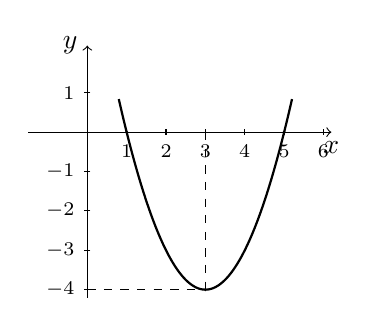
\begin{tikzpicture}[scale=0.5]
    \draw[->] (-1.5,0) -- (6.2,0) node[below] {$x$};
    \draw[->] (0,-4.2) -- (0,2.2) node[left] {$y$};
    \foreach \x in {1,2,3,4,5,6}
      \draw (\x,0.08)--(\x,-0.08) node[below] {\scriptsize $\x$};
    \foreach \y in {-4,-3,-2,-1,1}
      \draw (0.08,\y)--(-0.08,\y) node[left] {\scriptsize $\y$};
    \draw[smooth, samples=200, domain=0.8:5.2, thick] plot (\x, {(\x-3)^2-4});
    \fill (1,0) circle (1.2pt);
    \fill (5,0) circle (1.2pt);
    \fill (3,-4) circle (1.2pt);
    \draw[dashed] (3,0)--(3,-4);
    \draw[dashed] (0,-4)--(3,-4);
\end{tikzpicture}
